\chapter{Static analysis}
\label{static-analysis}\index{static analysis}\index{SA\see{static analysis}}\index{static code analysis|see{static analysis}}

\emph{Static (code) analysis (SA)} is defined as analyzing the code of a program (i.e., the source code, byte code or machine code) of a program without actually running it~\cite{chess-west}. The aim of static analysis is to find bugs, structural problems, code smells or to help in understanding the system that is analyzed. The opposite would be \emph{dynamic analysis}, e.g, unit testing or penetration testing on a running system.

\section{Static analysis for finding vulnerabilities}
\cite{chess-west} explains in detail how static analysis of code works and how it can be used to find bugs and vulnerabilities.

According to \cite{findbugs, evaluating}, tools for static code analysis can find real bugs in production software. \cite{coverity-report} elaborates on the numerous types of vulnerabilities that can be found using static analysis.

\section{Approaches to static analysis}
Generally, there are several approaches when doing static code analysis~\cite{comparison-of-bug-finding-tools, swaat, google-code-search}:

\begin{itemize}
 \item string pattern matching (with or without regular expressions)\index{string pattern matching}
 \item syntactic bug pattern detection (``style checking'')\index{style checking}\index{syntactic bug pattern detection}
 \item data-flow analysis (which relies on control-flow analysis) \index{data-flow analysis}\index{control-flow analysis}
 \item theorem proving (requires annotations with pre/post conditions)\index{theorem proving}
 \item model checking (requires code annotations that state the requirements)\index{model checking}
\end{itemize}

Pixy falls into the the data-flow analysis category.

\section{Tainted object propagation}
\label{tainting}\index{tainted object propagation}
\cite{finding-security-vulnerabilities} describes an approach to finding a class of vulnerabilities called \emph{tainted object propagation}. \cite{pixy-short, pixy-long, pixy-dissertation} apply this to PHP.

Tainted object propagation builds on data-flow analysis and traces where untrusted data comes into the system and where it is used. Pixy implements this approach.

The concepts of this approach are as following:
\paragraph{Sources} are the places where potentially malicious data comes in. In the example (figure \ref{fig:taint} on page \pageref{fig:taint}), the \texttt{\$\_GET} variable ``name'' is a source.\index{source}
\paragraph{Tainted} means that data is considered to be potentially dangerous.\index{tainting}
\paragraph{Sinks} are the places where the data is used and where tainted data could cause harm. In the example (figure \ref{fig:taint} on page \pageref{fig:taint}), the \texttt{echo} call is a sink.\index{sink}

\begin{figure}[!h]
  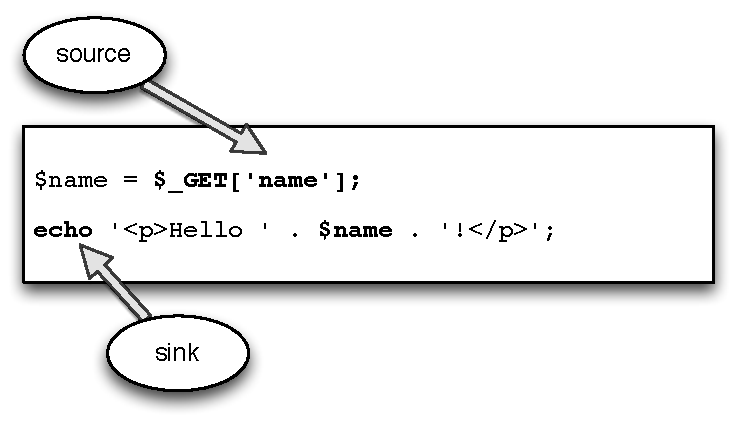
\includegraphics[scale=0.8]{images/taint}
  \caption{Tainted data can be traced on its way from the source to the sink.}
  \label{fig:taint}
\end{figure}

\paragraph{Sanitizing} tainted data from a source changes it so that it will not cause any harm when put into a sink. In the second example (figure \ref{fig:taint-and-clean} on page \pageref{fig:taint-and-clean}), the \texttt{htmlspecialchars} call sanitized the tainted data.\index{sanitizing}\index{sanitation|see{sanitizing}}

\begin{figure}[!h]
 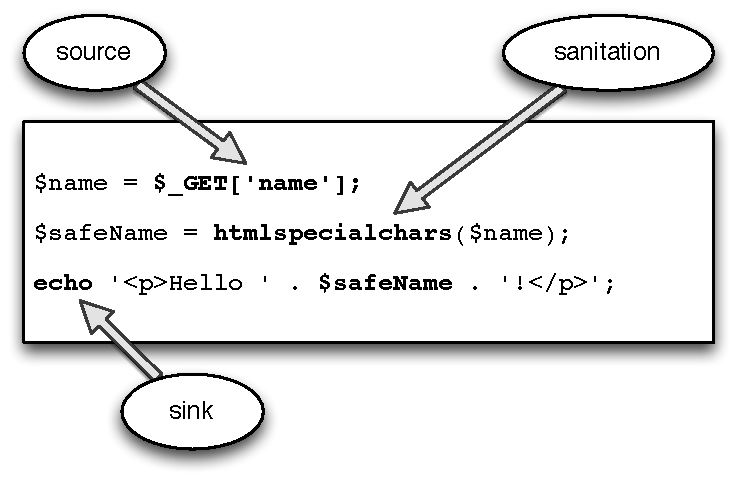
\includegraphics[scale=0.8]{images/taint-and-clean}
 \caption{Tainted data gets sanitized on its way from the source to the sink.}
 \label{fig:taint-and-clean}
\end{figure}

